%!TEX root = main.tex
%%%%%%%%%%%%%%%%%%%%%%%%%%%%%%%%%%%%%%%%%%%%%%%%%%%%%%%%%%%%%%%%%%%%%%%%%%%%%%%%

\section{Results}
\label{sec:results}

\begin{figure}[t]
\centering
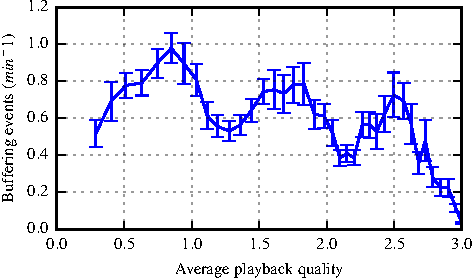
\includegraphics[width=0.95\linewidth]{figs/33qualityvstalling}%
\caption{Average playback quality versus stalling events}
\label{fig:qualityvsstalling}%
\end{figure}

Figure \ref{fig:qualityvsstalling} illustrates the relationship between the average quality level and the stalling events in the experiment result set.
For the average quality level, 0 is defined as \unit[100]{\%} of the segments are shown to the user in 144p. 3 is defined as \unit[100]{\%} of the segments are shown to the user in 480p.
The average quality levels are clustered using k-means and the error bars indicate the \unit[95]{\%} confidence interval of each cluster.
Two observations can be made from the figure. 
First, the lowest average quality level is 0.3 with about 0.5 switches per minute.
From this it follows that the player risks one stalling per two minutes in order to avoid showing only the lowest quality level in low bandwidth scenarios.
Second, the buffering events exhibit an oscillating behavior.
The oscillating behavior is consistent with observations made in \cite{sieber16sacrificing, casas2012youtube}.
The studies show that the performance of YouTube's adaptation algorithm depends on the ratio between video bit-rate and available bandwidth.
For certain ratios, the algorithm is able to efficiency use available bandwidth, i.e. there is only a low amount of redundant traffic and buffering.
Other ratios exhibit a high amount of redundant traffic and buffering ratio.
%There exists a fixed ratio of about three times the bit-rate compared to the network throughput (i.e. not application level throughput), where the time on that quality level is maximized, but also the quality switching and buffering ratio is increased.

In total, the pearson correlation shows a high correlation (-0.774) between average quality level and buffering events.

\subsection{Optimal Adaptation}

First, we will look at the adaptation of video resolution; second we will look at how many switches are expected to occur.

\begin{figure}[t]
\centering
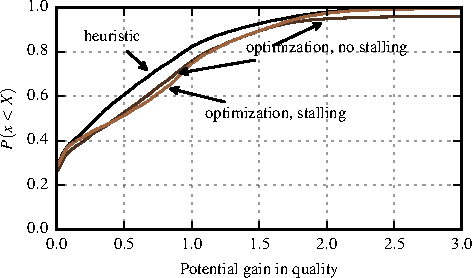
\includegraphics[width=0.5\textwidth]{figs/qualitygain_py}%
\caption{Distribution of the mean video quality in the measurement runs and highest achievable mean video quality according to the optimization problem from Section \ref{optadapt} and the heuristic from \cite{sieber16sacrificing}.}
\label{fig:opt}%
\end{figure}

Figure \ref{fig:opt} displays the CDF of the difference between the observed mean video quality and the optimal optimally achievable mean video quality.

Observations are as follows:
\begin{itemize}
\item about $30$ percent of runs are already at maximum quality and can therefore not be improved.
\item the optimization where initial delay is allowed allways leads to the highest quality.
\item However, the median of all three data sets is within $0.15$ of a quality of each other. This can be considered a minor difference.
\item In $56$ percent of the baseline runs stalling events did occur. In the figure, the \textit{opt(no stall)} demonstrates that theoretically, it would have been possible to avoid the stalling in $93$ percent of cases while increasing the quality in $30$ percent of cases. While \textit{opt(same stall)} shows that the mean quality could have been increased by adding an initial delay, this increase is not particularly high.
\item Further, while the heuristic leads to a worse result than \textit{opt(same stall)}, it has the advantage of being a less complex problem. This might outweigh the slightly better performance for practical purposes.
\end{itemize}

Finally, Figure \ref{fig:switches} shows the number of quality switches per minute. Here, both data sets that were created with the optimization approach lead to very similar results, which is why we only present the results for \textit{opt(no stall)}. While the number of switches is not of significant importance to the QoE in video streaming according to \cite{seufert2015survey}, continuous video quality switches lead to a low QoE \cite{liu2013user}. The heuristical approach and the optimization both lead to less than $2$ switches per minute in more than $80$ percent of cases which are acceptable values. However, the two-step approach for the optimization leads to some very high switching frequencies that might be problematic. This is because the two-step approach puts very high value on the optimization of the quality level and very little emphasis on the number of switches. Luckily, this problem can easily be averted by using a slightly different approach: In \cite{liotou2016enriching}, a method is proposed that combines both steps into one, allowing the number of switches to be emphasized higher at a negligibly low cost of quality.

\begin{figure}[t]
\centering
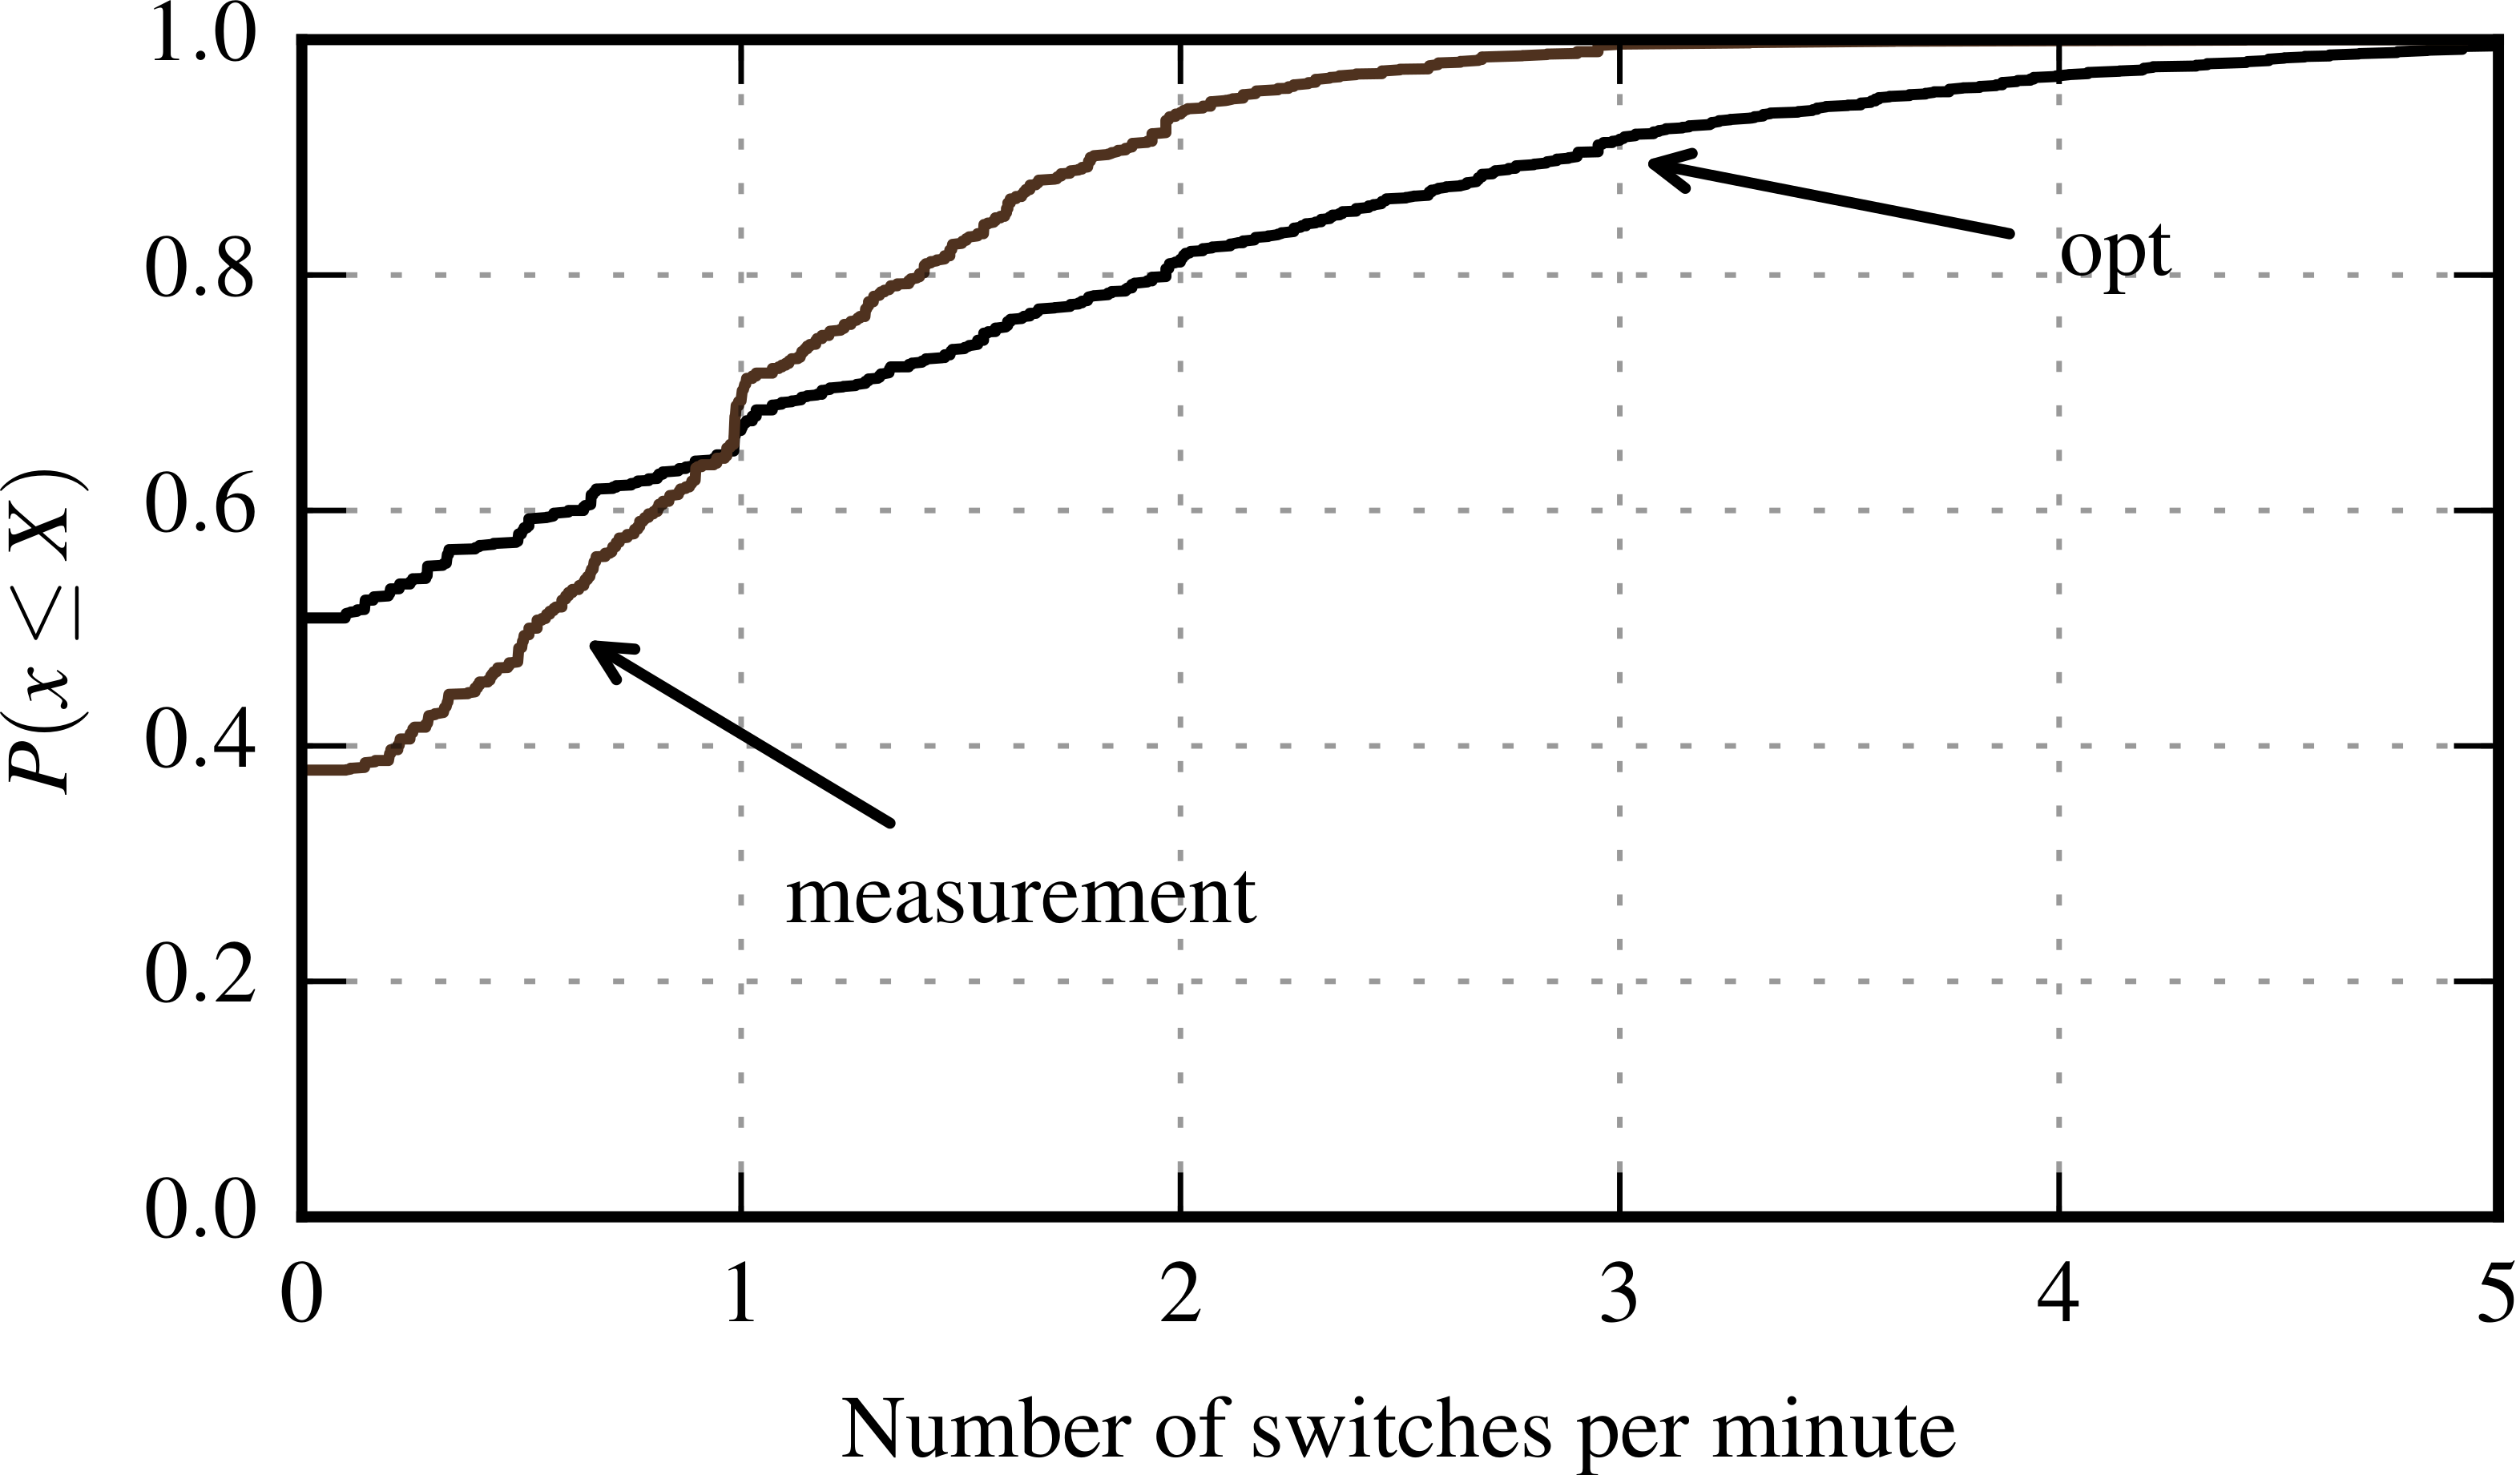
\includegraphics[width=0.5\textwidth]{figs/switches_py}%
\caption{Distribution of the number of switches per minute for the heuristic and the optimization}
\label{fig:switches}%
\end{figure}

